\documentclass[tikz,border=5pt]{standalone}
\usetikzlibrary{calc, arrows.meta, decorations.pathmorphing}

\begin{document}

% Figure 05: Hyperbolic Polytope (Fundamental Chamber)
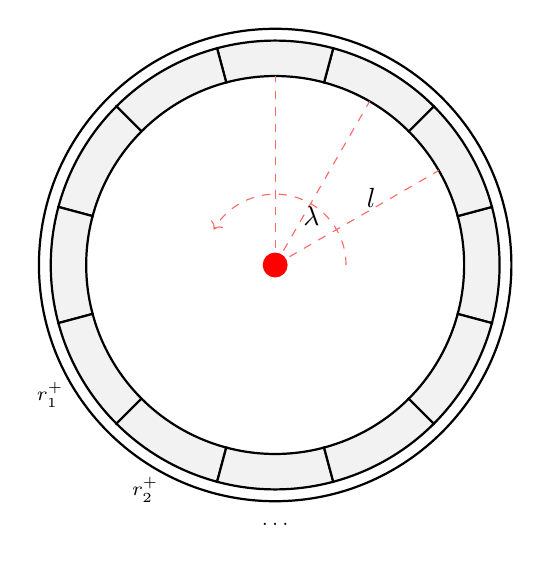
\begin{tikzpicture}[scale=3]
    % Draw the main circular boundary (unit disk)
    \draw[thick] (0,0) circle (1);

    % Draw the "scalloped" lobed interior boundary
    % Approximated with a series of arcs
    \foreach \ang in {0, 30, ..., 330} {
        \draw[thick, fill=gray!10] 
            ({\ang-15}:0.95) arc ({\ang-15}:{\ang+15}:0.95) 
            -- ({\ang+15}:0.8) arc ({\ang+15}:{\ang-15}:0.8) -- cycle;
    }

    % Labels for lobes
    \node[font=\scriptsize] at (210:1.1) {$r_1^+$};
    \node[font=\scriptsize] at (240:1.1) {$r_2^+$};
    \node[font=\scriptsize] at (270:1.1) {$\dots$};

    % Interior structure (Dashed lines)
    \draw[dashed, red!60] (0,0) -- (30:0.8) node[midway, above right, black] {$l$};
    \draw[dashed, red!60] (0,0) -- (60:0.8);
    \draw[dashed, red!60] (0,0) -- (90:0.8);
    \draw[dashed, red!60, ->] (0:0.3) arc (0:150:0.3) node[midway, below right, black] {$\lambda$};

    % Central node (Red dot)
    \fill[red] (0,0) circle (1.5pt);

\end{tikzpicture}

\end{document}
